% Straight up stealing preamble from Eli Holmes 
%%%%%%%%%%%%%%%%%%%%%%%%%%%%%%%%%%%%%%START PREAMBLE THAT IS THE SAME FOR ALL EXAMPLES
\documentclass{article}

%Required: You must have these
\usepackage{Sweave}
\usepackage{graphicx}
\usepackage{tabularx}
\usepackage{hyperref}
\usepackage{natbib}
\usepackage{pdflscape}
\usepackage{array}
\usepackage{gensymb}
%\usepackage[backend=bibtex]{biblatex}
%Strongly recommended
  %put your figures in one place
%\SweaveOpts{prefix.string=figures/, eps=FALSE} 
%you'll want these for pretty captioning
\usepackage[small]{caption}

\setkeys{Gin}{width=0.8\textwidth}  %make the figs 50 perc textwidth
\setlength{\captionmargin}{30pt}
\setlength{\abovecaptionskip}{10pt}
\setlength{\belowcaptionskip}{10pt}
% manual for caption  http://www.dd.chalmers.se/latex/Docs/PDF/caption.pdf

%Optional: I like to muck with my margins and spacing in ways that LaTeX frowns on
%Here's how to do that
 \topmargin -1.5cm        
 \oddsidemargin -0.04cm   
 \evensidemargin -0.04cm  % same as oddsidemargin but for left-hand pages
 \textwidth 16.59cm
 \textheight 21.94cm 
 %\pagestyle{empty}       % Uncomment if don't want page numbers
 \parskip 7.2pt           % sets spacing between paragraphs
 %\renewcommand{\baselinestretch}{1.5} 	% Uncomment for 1.5 spacing between lines
\parindent 0pt% sets leading space for paragraphs
\usepackage{setspace}
%\doublespacing

%Optional: I like fancy headers
%\usepackage{fancyhdr}
%\pagestyle{fancy}
%\fancyhead[LO]{How do climate change experiments actually change climate}
%\fancyhead[RO]{2016}
 
%%%%%%%%%%%%%%%%%%%%%%%%%%%%%%%%%%%%%%END PREAMBLE THAT IS THE SAME FOR ALL EXAMPLES

%Start of the document
\begin{document}

%\SweaveOpts{concordance=TRUE}
 \bibliographystyle{/Users/aileneettinger/citations/Bibtex/styles/amnat.bst}
\title{Spatial and temporal shifts in photoperiod with climate change} % perspective paper for OSPREE analyses

\author{A.K. Ettinger, D. Buonaiuto, C. Chamberlain, I. Morales-Castilla, E. Wolkovich}
%\date{\today}%do we need to also add any of the following: D. Flynn, T. Savas, J. Samaha, E. Forrestel? 
\maketitle  %put the fancy title on
%\tableofcontents      %add a table of contents
%\clearpage
%%%%%%%%%%%%%%%%%%%%%%%%%%%%%%%%%%%%%%%%%%%%%%%%%%%
\begin{enumerate}
\item \textit{Introduction}
\begin{enumerate}
\item Photoperiod is a critical cue used by organisms to synchronize their activities with seasonal climatic changes (add other citations- there are many possibilities! if you have favorites, please add along with 1-2 words of what the activity is)\citep[e.g.,][]{Hsu:2011,Singh:2017,Basler:2012,Flynn:2018}.
\item As species undergo climate change-induced shifts in space and/or time, the daylength they experience will be altered. 
\item Many experiments have altered photoperiod, often interacting with temperature changes; however, photoperiod treatments in these experiments are not typically designed to be applied to climate change forecasting. 
\item Here, we ask: 
\begin{enumerate}
\item How will climate change alter the photoperiod experienced by organisms, given observed climate change-induced biological shifts, both spatially and temporally?
\item What are the implications of these altered photoperiods for forecasts of climate change impacts?
\item Can the large quantity of experiments altering photoperiod be applied to forecasting biological implications of climate change (i.e., do they occur at the appropriate scale)?
\end{enumerate}
\end{enumerate}

\item\textit{How will climate change alter the photoperiod experienced by organisms?}
\begin{enumerate}
\item Spatial shifts in species ranges and temporal shifts in species phenology and activity will alter the photoperiods experienced by organisms under climate change.
\item  To date, most work has focused on how spatial range shifts with climate change will affect photoperiod \citep{saikkonen2012}, but temporal shifts are actually likely to yield bigger changes in experienced photoperiod than spatial shifts (Figure \ref{fig:spacetime}).
\item Shifts in photoperiod may vary with latitude and time of year, especially since phenology varies with latitude (Figure \ref{fig:greenup}).
\item Photoperiod sensitivity can also vary with latitude \citep{Howe:1996,saikkonen2012,Partanen:2005aa,Vihera-Aarnio:2006aa,Caffarra:2011b,gauzere2017}, so it is unclear how these two things interact. Cat has added a text file to the latitude analysis folder that summarizes papers that have looked at latitudinal effects on photoperiod.
\end{enumerate}
\item\textit{What are the implications of these altered photoperiods for forecasts of climate change impacts?}
\begin{enumerate}
\item Phenology will be altered, given that daylength is known to affect vegetative growth, cell elongation, and budburst \citep{Linkosalo:2006aa,erwin1998,sidaway2010, Hsu:2011}.
\item It has been proposed that photoperiod may eventually become a limiting factor, constraining the ability of trees to shift their phenology with warming \citep{koerner2010b,vitasse2013, Morin:2010aa}. 
\item Interactions between photoperiod and forcing and chilling could result in muted or exaggerated phenological shifts, compared to what would be expected based on temperature change alone. Say something about crossing thresholds of daylength and the "external coincidence model" for photoperiod control \citep{bastow2002,kobayashi2007,andres2012,Singh:2017}?
\item Effects of photoperiod on forecasting of biological impacts of climate change needs additional investifation. In some forecasting methods (e.g. species distirbution modelling), the role of photoperiod is largely ignored (i think this is true? add some citations). In other cases, photoperiod is incorporated into foreacasts, along with other variables such as evaporative demand, and temperature \citep [e.g. ED] []{jolly2005, medvigy2013}. These models need to be more widely tested, e.g. in different ecosystems/species, and need to incorporate recent findings about the role of photoperiod in phenology.     
\end{enumerate}
\item\textit{Can existing experiments be applied to forecasting?}
\begin{enumerate}
\item In some cases, yes, experiments manipulate photoperiod at relevant scales (Figure \ref{fig:photomap}, Table \ref{table:phototreats}).
\item However, most experiments manipulate photoperiod much more dramatically than will occur with climate change (Figures \ref{fig:photomap}, \ref{fig:fagus},\ref{fig:quercus}, but see \citep{Basler:2012}), so it is difficult to extrapolate findings. (This may not be true for all latitudes- for example high latitudes experience more dramatic changes in photoperiod across the year.)
\item There is a great need to better understand exactly how photoperiod acts as a cue. The divergent effects of photoperiod observed across studies (e.g., Figure \ref{fig:photocurve}) suggests that photoperiod interacts with other environmental drivers, such as chilling and forcing, to affect phenology and other activities. However, exactly how it interacts with temprature to break dormancy, as well as the type of response it ellicits (e.g., linear versus non-linear threshold) is unclear. 
\end{enumerate}
\item\textit{Conclusions}
\begin{enumerate}
\item Organisms may experience large changes to the photoperiod they experience, under climate change, even if they do not shift their ranges spatially.
\item More studies needed with fine-scale changes in photoperiod.
\end{enumerate}
\end{enumerate}

\section* {To do:}
\begin{enumerate}
\item Make Table of studies testing if photoperiod varies by latitudinal origin- cat started on this (Table 2)?
\item Update table/map to use 3 ER studies.
\end{enumerate}
\section* {Random notes that may be useful:}
\begin {enumerate}
\item Bradshaw and Holzapfel (2001) showed that the pitcher plant mosquito,
Wyeomyia smithii, has evolved a shorter critical photoperiod in association with a
longer growing season. Northern populations of this mosquito now use a shorter
day-length cue to enter winter diapause, doing so later in the fall than they did
24 years ago.
\item Decreasing day-length is the main environmental cue inducing growth cessation and bud set in many perennial plants, including poplar 
\begin{enumerate}

\item Lagercrantz U: At the end of the day: a common molecular mechanism for photoperiod responses in plants?. J Exp Bot. 2009, 60: 2501-2515. 10.1093/jxb/erp139.
\item Howe GT, Gardner G, Hackett WP, Furnier GR: Phytochrome control of short-day-induced bud set in black cottonwood. Physiol Plant. 1996, 97: 95-103. 10.1111/j.1399-3054.1996.tb00484.x.
\end{enumerate}

\item Response to photoperiod is under strong genetic control 
\begin{enumerate}
\item Bradshaw HD, Stettler RF: Molecular genetics of growth and development in Populus. IV. Mapping QTLs with large effects on growth, form, and phenology traits in a forest tree. Genetics. 1995, 139: 963-973.
\item Keller SR, Soolanayakanahally RY, Guy RD, Silim SN, Olson MS, Tiffin P: Climate-driven local adaptation of ecophysiology and phenology in balsam poplar, Populus balsamifera L. (Salicaceae). Am J Bot. 2011, 98: 99-108. 10.3732/ajb.1000317.
\item Weih M: Intensive short rotation forestry in boreal climates: present and future perspectives. Can J Forest Res. 2004, 34: 1369-1378. 10.1139/x04-090.
\end{enumerate}
\end {enumerate}
\bibliography{/Users/aileneettinger/git/ospree/refs/ospreebibplus}
\clearpage
\section* {Tables}
% latex table generated in R 3.4.2 by xtable 1.8-2 package
% Fri Aug  3 15:34:11 2018
\begin{table}[ht]
\centering
\caption{\textbf{Growth chamber experiments and their photoperiod treatments}, compared to the spatial and temporal shifts required for organisms to experiments photoperiod changes equivalent to those treatments. For shifts in space, `ER' indicates that the photoperiod treatments exceeds the change of photoperiod from moving up to 40 degrees latitudinally on June 21. For shifts in time, `ER' indicates that the range of photoperiod treatments exceeds the change in daylengths at that latitude during the entire year. `max NA' indicates that the maximum daylength treatment does not exist at that latitude; `min NA'indicates that the minimum daylength treatment does not exist at that latitude.} 
\label{table:phototreats}
\begin{tabular}{|p{0.18\textwidth}|p{0.15\textwidth}|p{0.08\textwidth}|p{0.08\textwidth}|p{0.08\textwidth}|p{0.06\textwidth}|p{0.06\textwidth}|p{0.12\textwidth}|}
  \hline
idstudy & continent & lat & long & day\_range & delta & space & time \\ 
  \hline
ashby62\_exp1 & north america & 42.99 & -89.41 & 8-16 & 4.00 & 18.2 & min NA (9) \\ 
  basler14\_exp1 & europe & 46.31 & 8.27 & 9.2-16 & 1.00 & 6 & -22 \\ 
  caffarra11b\_exp2 & europe & 52.32 & -6.93 & 10-16 & 2.00 & 7.5 & -30 \\ 
  devries82\_exp1 & europe & 51.98 & 5.66 & 8-24 & 16.00 & ER & ER \\ 
  falusi90\_exp1 & europe & 46.03 & 10.75 & 9-13 & 4.00 & 16 & -82 \\ 
  falusi96\_exp3 & europe & 38.27 & 15.99 & 9-13 & 4.00 & 21.6 & -111 \\ 
  ghelardini10\_exp1 & europe & 43.72 & 11.37 & 8-16 & 8.00 & 21.9 & ER \\ 
  heide05\_exp1 & europe & 56.18 & -4.32 & 10-24 & 14.00 & ER & ER \\ 
  heide08\_exp1 & europe & 48.40 & 11.72 & 10-24 & 14.00 & ER & ER \\ 
  heide11\_exp1 & europe & 59.67 & 10.67 & 10-20 & 10.00 & ER & max NA (18.7) \\ 
  heide12\_exp1 & europe & 56.50 & -3.06 & 10-24 & 5.00 & 8.9 & -64 \\ 
  heide15\_exp2 & europe & 56.50 & -3.06 & 10-15 & 1.00 & 3.2 & -13 \\ 
  heide93\_exp1 & europe & 59.50 & 10.77 & 8-24 & 16.00 & ER & ER \\ 
  heide93a\_exp1 & europe & 59.67 & 10.83 & 8-24 & 16.00 & ER & ER \\ 
  heide93a\_exp3 & europe & 47.50 & 7.60 & 13-16 & 1.00 & 5.7 & -18 \\ 
  howe95\_exp1 & north america & 40.55 & -124.10 & 9-24 & 2.00 & 13.1 & -64 \\ 
  laube14a\_exp1 & europe & 48.40 & 11.71 & 8-16 & 4.00 & 14.3 & -87 \\ 
  myking95\_exp1 & europe & 56.10 & 9.15 & 8-24 & 16.00 & ER & ER \\ 
  myking97\_exp1 & europe & 59.67 & 10.77 & 12-24 & 12.00 & ER & max NA (18.7) \\ 
  nienstaedt66\_exp1 & north america & 44.17 & -103.92 & 8-20 & 12.00 & ER & ER \\ 
  okie11\_exp1 & north america & 32.12 & -83.12 & 0-12 & 12.00 & ER & ER \\ 
  partanen01\_exp1 & europe & 61.93 & 26.68 & 6-16 & 10.00 & ER & -105 \\ 
  partanen05\_exp1 & europe & 61.82 & 29.32 & 5-20 & 5.00 & ER & -67 \\ 
  partanen98\_exp1 & europe & 60.03 & 23.05 & 8.66-12 & 3.34 & 5.1 & -37 \\ 
  pettersen71\_exp1 & europe & 59.66 & 10.77 & 10-24 & 2.00 & 4 & -23 \\ 
  Sanz-Perez09\_exp1 & europe & 40.40 & -3.48 & 10-16 & 6.00 & 23.6 & ER \\ 
  skuterud94\_exp1 & europe & 61.50 & 24.33 & 8-24 & 16.00 & ER & ER \\ 
  viheraaarnio06\_exp1 & europe & 60.45 & 24.93 & 16-17 & 1.00 & 2.1 & -12 \\ 
  viheraaarnio06\_exp1 & europe & 67.73 & 24.93 & 20-21 & 1.00 & ER & -5 \\ 
  viheraaarnio06\_exp2 & europe & 60.45 & 24.93 & 15-19 & 4.00 & 5.1 & -62 \\ 
  viheraaarnio06\_exp2 & europe & 67.73 & 24.93 & 22-23 & 1.00 & ER & -3 \\ 
  worrall67\_exp 3 & north america & 41.31 & -72.93 & 8-16 & 8.00 & 24.3 & ER \\ 
  zohner16\_Exp1 & europe & 48.16 & 11.50 & 8-16 & 8.00 & ER & ER \\ 
   \hline
\end{tabular}
\end{table}\clearpage
\section* {Figures}
\begin{figure}[p]
\centering
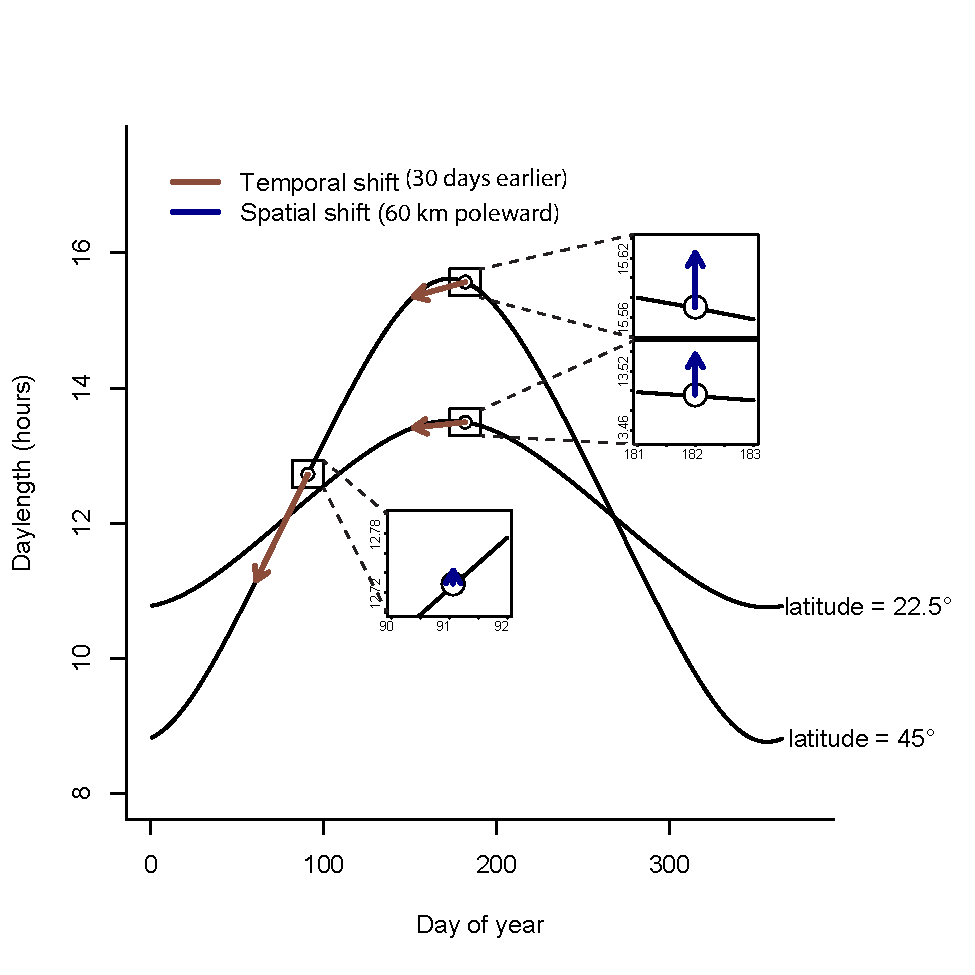
\includegraphics{/Users/aileneettinger/git/ospree/analyses/photoperiod/figures/photo_spacetime_v2.pdf} %
\caption{\textbf{Photoperiod varies with latitude and throughout the year}, such that temporal shifts in activity yield larger changes in experienced photoperiod compared with spatial shifts. Here, we show this variation at two latitudes, using hypothetical rates of spatial and temporal shifts: 30 days earlier for temporal shifts, and 0.5 degrees poleward for spatial shifts. These shifts, which are similar to observed average rates (e.g., Parmesan et. al 2006, Chen et al 2011), highlight the greater magnitude in daylength changes close to the equinox (e.g., DOY 91), versus close to the summer solcstice (e.g., DOY 182).}
 \label{fig:spacetime}%
 \end{figure}
 
\begin{figure}[p]
\centering
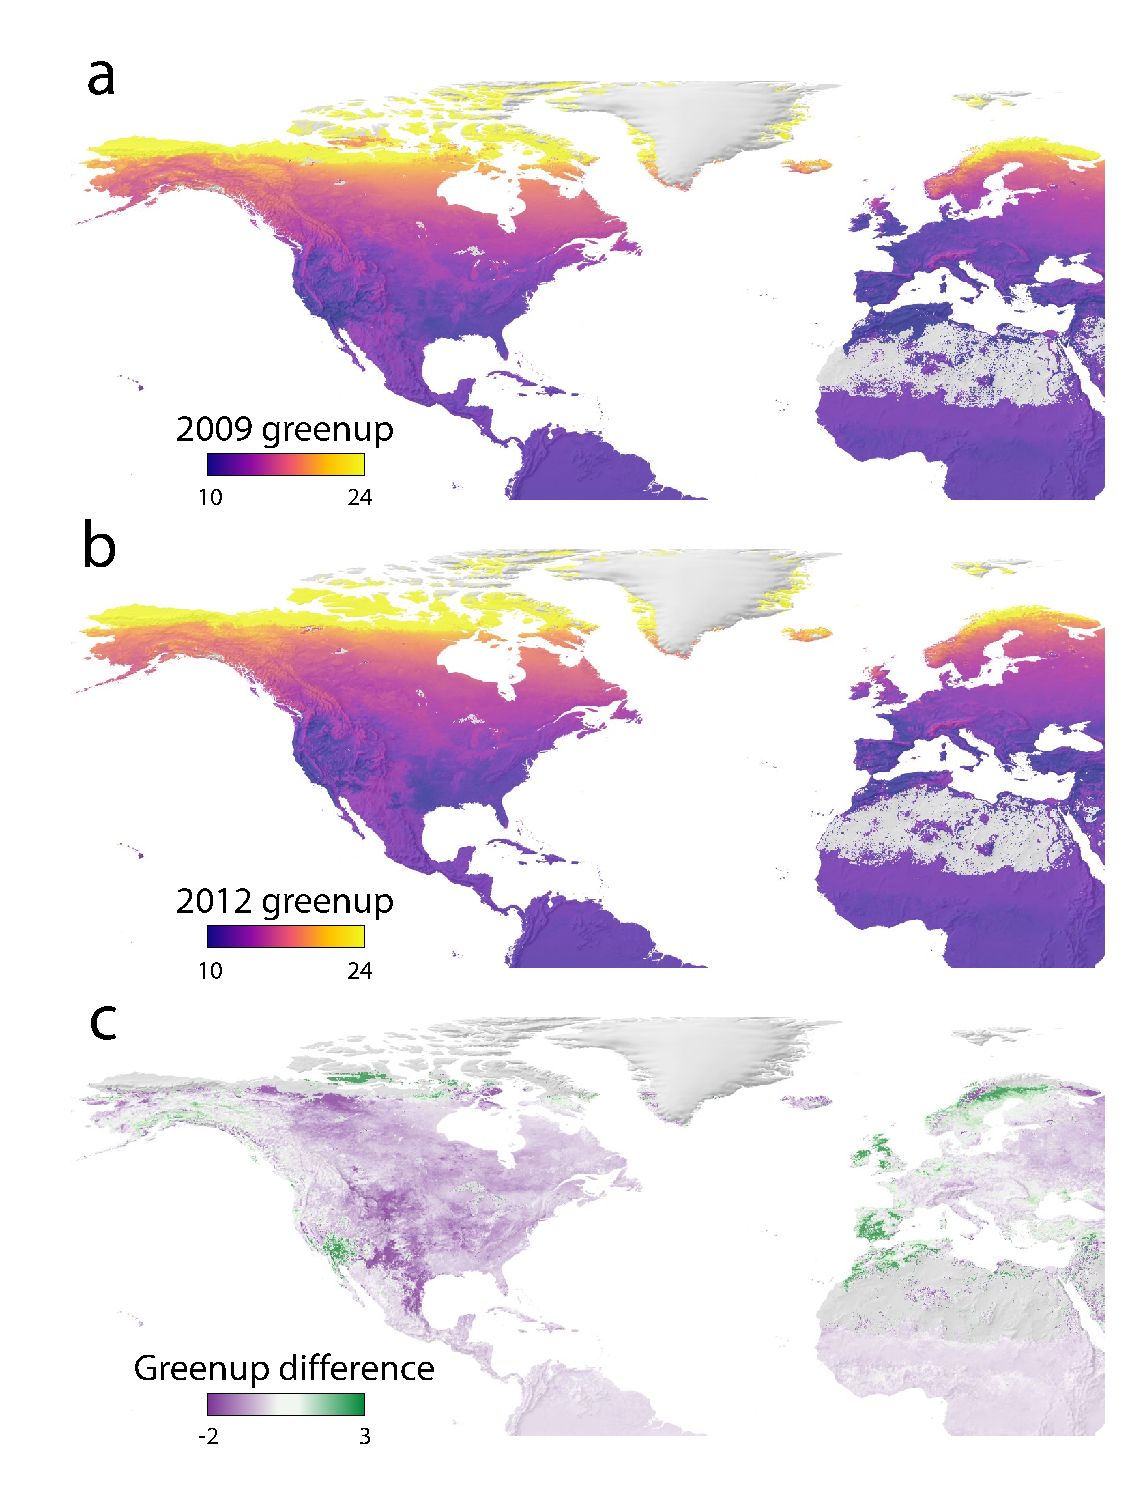
\includegraphics{/Users/aileneettinger/git/ospree/docs/photoperiod/figures/Greenup_.pdf} %2009 greenup
\caption{\textbf{The photoperiod on the green up date (start of spring) varies over space} and among years. Hours of daylight on the date of spring green up from MODIS satilite data across North America and Europe for an average (a) and  early (b) North American start of spring. The differences between the years are shown in (c). }
 \label{fig:greenup}%
 \end{figure}
\begin{figure}[p]
\centering
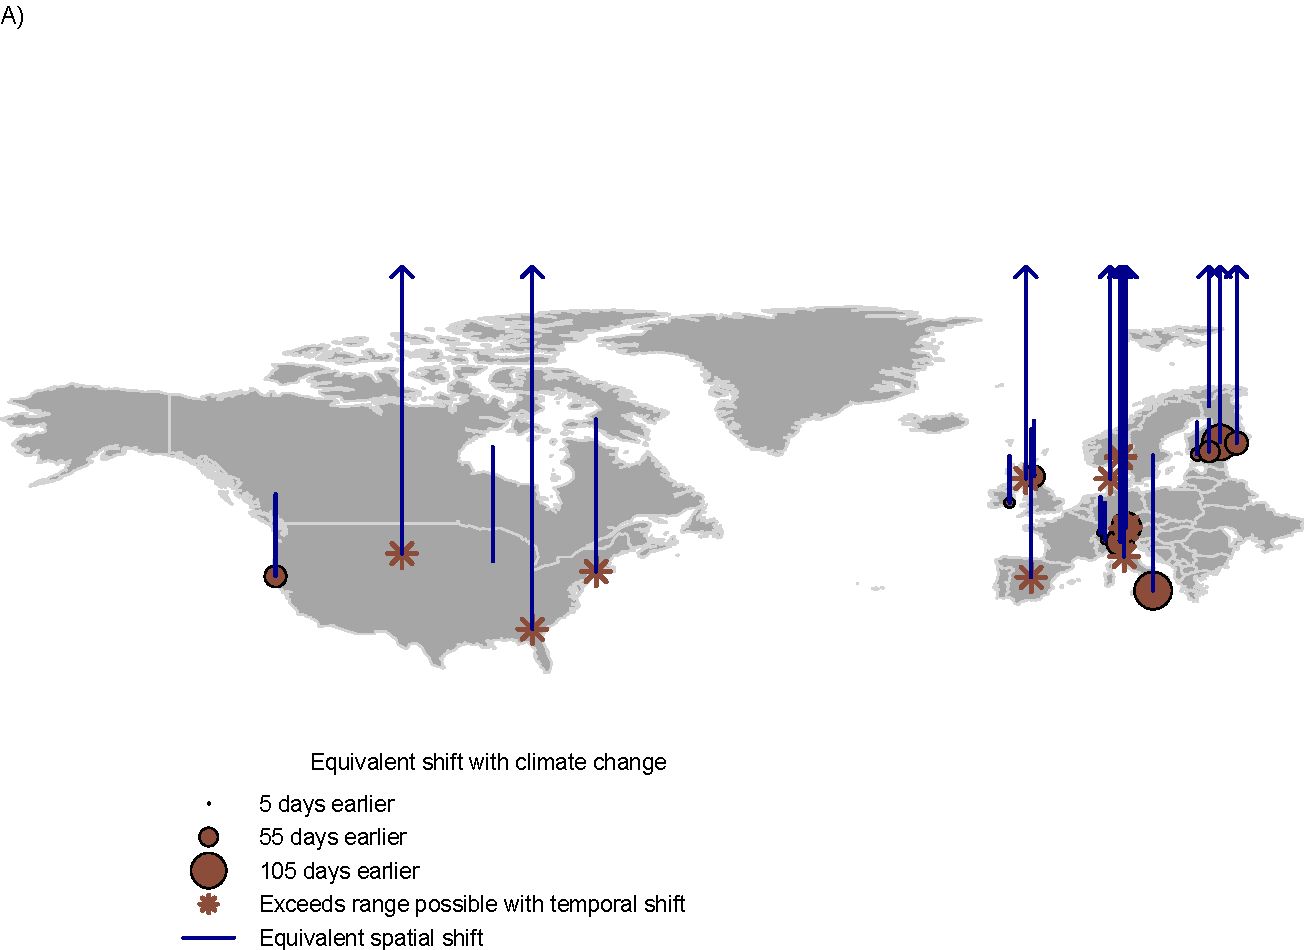
\includegraphics{/Users/aileneettinger/git/ospree/analyses/photoperiod/figures/ospree_photopmap.pdf} 
\caption{\textbf{OSPREE experiments that manipulate photoperiod}, and their equivalent spatial and temporal shifts, mapped (A), and graphed (B-C). Observed rates (dashed gray lines) 16.9 kilometers per decade (or approximately 1.5 degrees in 100 years) for spatial shifts (Chen et al. 2011) and 2.3 days per decade (or 23 days in 100 years) for temporal shifts (Parmesan and Yohe 2003).}
 \label{fig:photomap}
 \end{figure}


 
\begin{figure}[p]
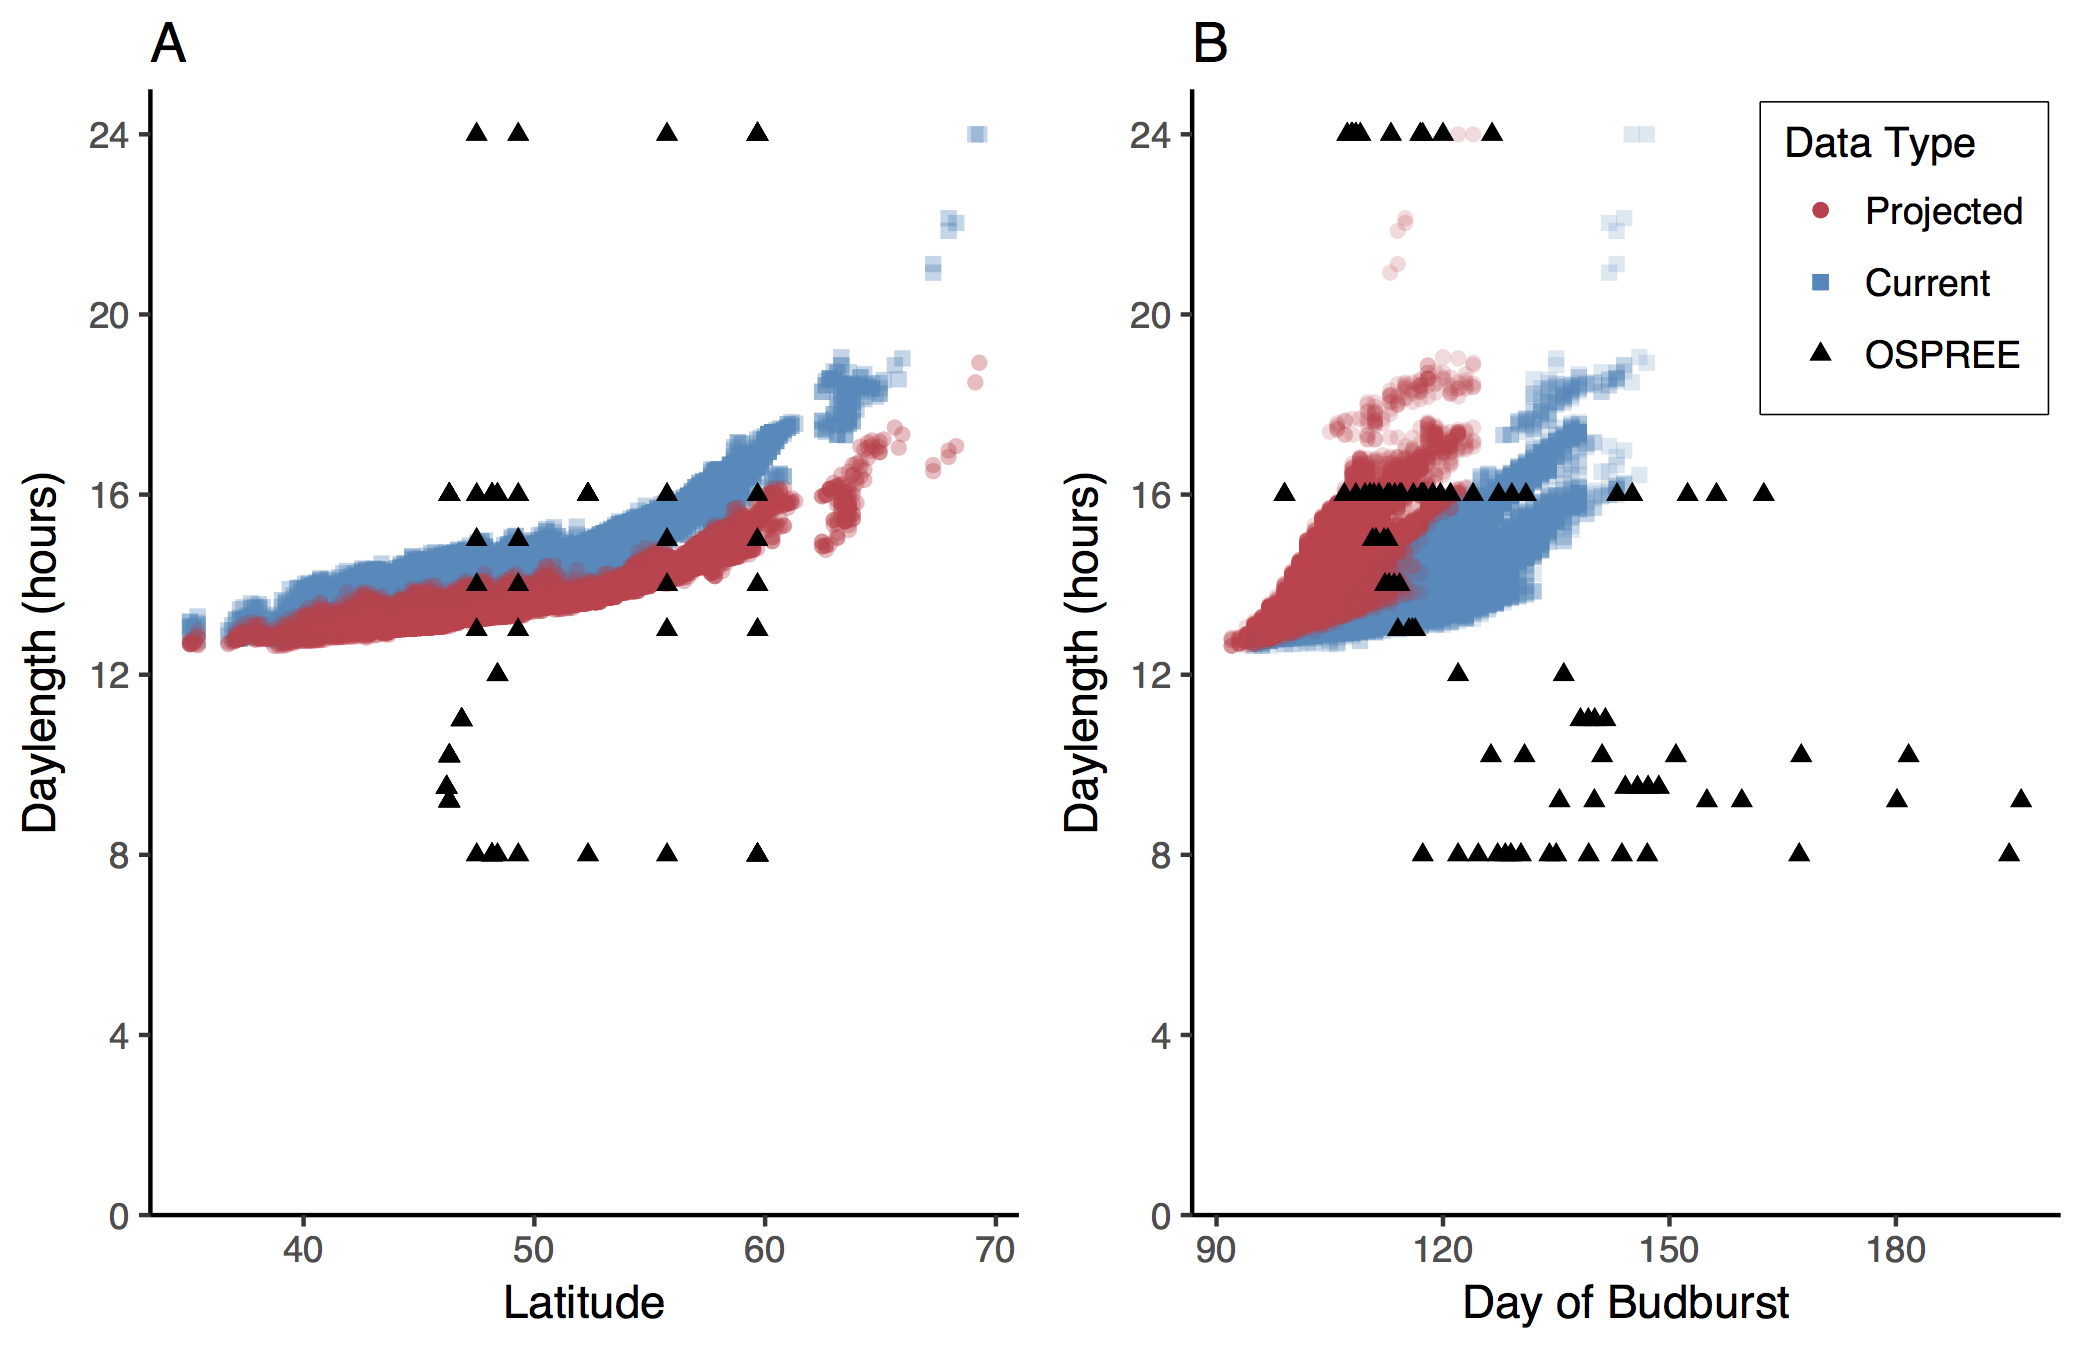
\includegraphics{/Users/aileneettinger/git/ospree/analyses/photoperiod/figures/2D_fagus_actual.png} 
\caption{\textbf{Experimental treatments of daylength in the OSPREE database, shown by latitude (A) and by day of budburst (B)} for \textit{Fagus sylvatica}. For comparison, we show the daylength when budburst occurs in its current and projected ranges (A) and in its current range only, with expected shifts in phenology (B). Estimates and projections are from Phenofit \citep{duputie2015}}
 \label{fig:fagus}
 \end{figure}
 
\begin{figure}[p]
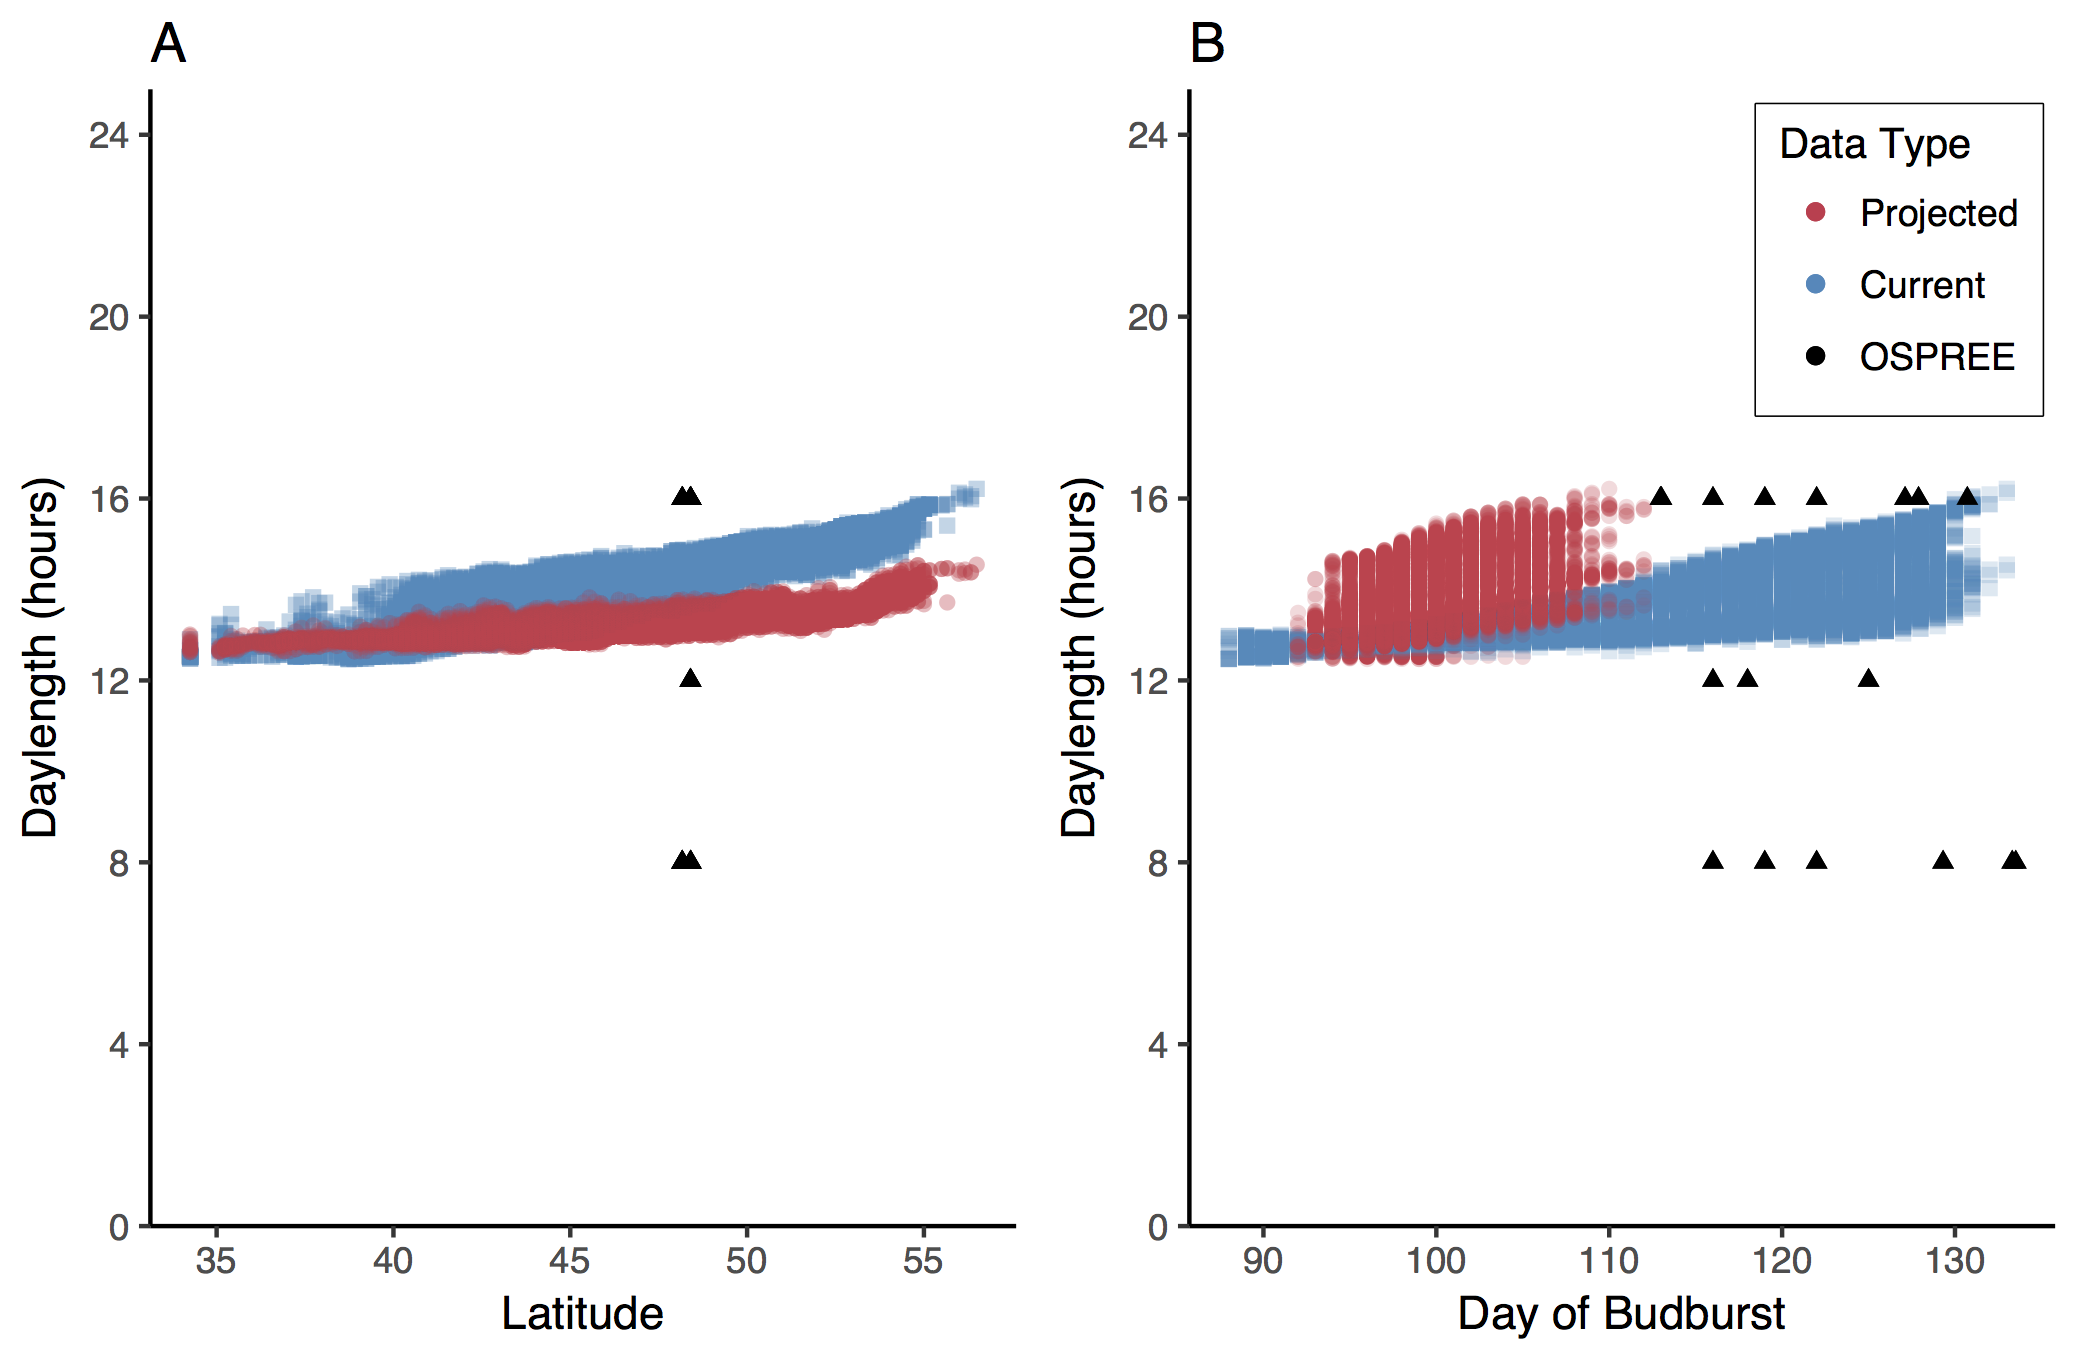
\includegraphics{/Users/aileneettinger/git/ospree/analyses/photoperiod/figures/2D_quercus_actual.pdf} 
\caption{\textbf{Experimental treatments of daylength in the OSPREE database, shown by latitude (A) and by day of budburst (B)} for \textit{Quercus robur}. For comparison, we show the daylength when budburst occurs in its current and projected ranges (A) and in its current range only, with expected shifts in phenology (B). Estimates and projections are from Phenofit \citep{duputie2015}.}
 \label{fig:quercus}
 \end{figure}
 
 \begin{figure}[p]
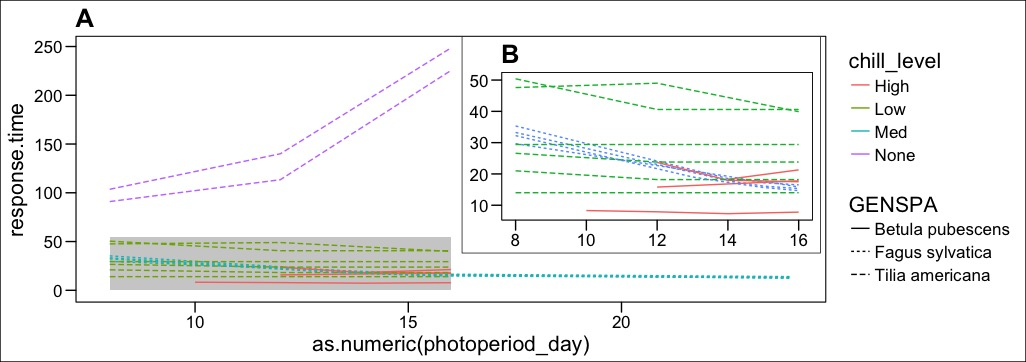
\includegraphics{/Users/aileneettinger/git/ospree/analyses/photoperiod/figures/New_photo_curve.jpeg} 
\caption{\textbf{Plant responses to changes in daylength vary across species and populations, and with the amount of chilling recieved}.}
 \label{fig:photocurve}
 \end{figure}
%%%%%%%%%%%%%%%%%%%%%%%%%%%%%%%%%%%%%%%%
\end{document}
%%%%%%%%%%%%%%%%%%%%%%%%%%%%%%%%%%%%%%%%
